\documentclass[tikz, border=7pt]{standalone}
\usepackage{tikz}
\usepackage{tkz-euclide}
\usepackage{amsmath}
\usepackage{amsfonts}
\usepackage{amssymb}


\newcommand\Mydiv[2]{%
$\strut#1$\kern.25em\smash{\raise.3ex\hbox{$\big)$}}$\mkern-8mu
        \overline{\enspace\strut#2}$}
\begin{document}
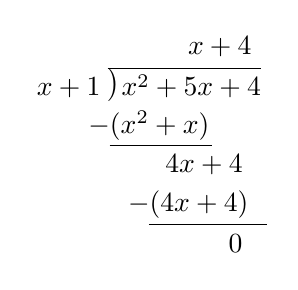
\begin{tikzpicture}

\node (c) at (0.5,3) {\Mydiv{x+1}{x^2+5x+4}};
\node (c) at (0.5,2.5) {$-(x^2+x)$};
\draw (-0, 2.25) -- (1.3,2.25);
\node (c) at (1.2,2) {$4x+4$};
\node (c) at (1,1.5) {$-(4x+4)$};
\draw (0.5, 1.25) -- (2,1.25);
\node (c) at (1.6,1) {$0$};

\node (c) at (1.4,3.5) {$x+4$};



\end{tikzpicture}
\end{document}
